\documentclass{article}
\usepackage {inputenc, fullpage, listings, amsmath, graphicx, wasysym, cancel}

\parindent 0pt

\title{%
   CSc 320: Foundations of Computer Science (Summer 2022)\\
    \Large Alex Holland \\
    Assignment 3\\
    }
\date{}

\begin{document}

\maketitle

{\bf Question 1}\\
\begin{equation*} 
\begin{split}
   & \{q_0,q_1\} \; \cancel{\{q_1,q_2\}} \; \{q_2,q_3\} \; \cancel{\{q_3,q_4\}} \; \cancel{\{q_4,q_5\}} \; \cancel{\{q_5,q_6\}} \; \{q_6,q_7\} \\
   & \cancel{\{q_0,q_2\}} \; \cancel{\{q_1,q_3\}} \; \cancel{\{q_2,q_4\}} \; \{q_3,q_5\} \; \{q_4,q_6\} \; \cancel{\{q_5,q_7\}} \\
   & \cancel{\{q_0,q_3\}} \; \{q_1,q_4\} \; \{q_2,q_5\} \; \cancel{\{q_3,q_6\}} \; \{q_4,q_7\} \\
   & \{q_0,q_4\} \; \cancel{\{q_1,q_5\}} \; \cancel{\{q_2,q_6\}} \; \cancel{\{q_3,q_7\}} \\
   & \cancel{\{q_0,q_5\}} \; \{q_1,q_6\} \; \cancel{\{q_2,q_7\}} \\
   & \{q_0,q_6\} \; \{q_1,q_7\} \\
   & \{q_0,q_7\} \\
\end{split}
\end{equation*}

\begin{equation*} 
\begin{split}
   & \cancel{\{q_0,q_1\}} \; \cancel{\{q_1,q_4\}} \; \{q_2,q_3\} \; \{q_3,q_5\} \; \{q_4,q_6\} \; \cancel{\{q_6,q_7\}} \\
   & \cancel{\{q_0,q_4\}} \; \cancel{\{q_1,q_6\}} \; \{q_2,q_5\} \;\;\;\;\;\;\;\;\;\;\;\;\;\; \cancel{\{q_4,q_7\}}\\
   & \cancel{\{q_0,q_6\}} \; \{q_1,q_7\} \\
   & \cancel{\{q_0,q_7\}} \\
\end{split}
\end{equation*}

\begin{equation*} 
\begin{split}
   & \cancel{\{q_1,q_7\}} \cancel{\{q_2,q_3\}} \; \{q_3,q_5\} \; \{q_4,q_6\} \\
   & \;\;\;\;\;\;\;\;\;\;\;\; \cancel{\{q_2,q_5\}}
\end{split}
\end{equation*}

\begin{equation*} 
\begin{split}
   & \{q_3,q_5\} \{q_4,q_6\} \\\\
   & q_3 \sim q_5, q_4 \sim q_6\\
\end{split}
\end{equation*}

\begin{center}
    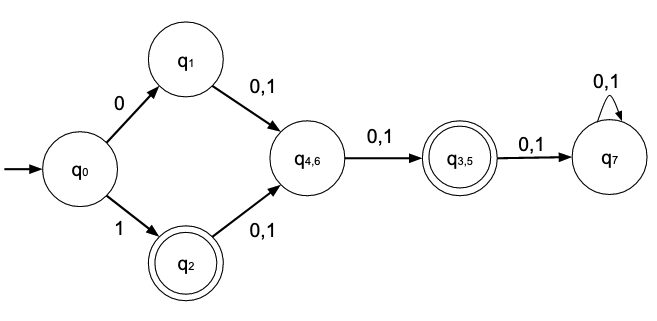
\includegraphics[width=0.8\textwidth]{1.png}
\end{center}

\break
{\bf Question 2}\\
Assume for $L = \{w \in \{0,1\}^* | w = 0^i0101^{2i}, i \geq 0 \}$, that $L$ is regular.\\
Let $s = 0^p0101^{2p}: s \in L \text{ and } |s| \geq p$\\
We can split the string s into 3 parts $s = xyz$ satisfying the conditions:

\begin{enumerate}
  \item $xy^iz \in L$ for each $i \geq 0$
  \item $|y| > 0$
  \item $|xy| \leq p$
\end{enumerate}

Observe all decomposition's of $s$:

\begin{itemize}
  \item $x = 0^\alpha$ where $\alpha \geq 0$
  \item $y =  0^\beta$ where $\beta \geq 1$ $(\alpha + \beta \leq p)$
  \item $0^{p - \alpha - \beta}0101^{2p}=0^{p-\alpha - \beta+1}101^{2p}$
\end{itemize}

Choose one $i$ such that $xy^iz \notin L$.\\ 
Let's pick $i = 2$:\\
\begin{equation*} 
\begin{split}
   xy^2z &= 0^\alpha 0^\beta 0^\beta 0^{p-\alpha - \beta + 1}101^{2p}\\
   &= 0^{p + \beta + 1}101^{2p}\\
\end{split}
\end{equation*}

$0^{p + \beta + 1}101^{2p} \in L$ iff $p+\beta+1=2p$\\
We can simplify $p + \beta + 1 = 2p$ to $\beta + 1 = p$\\
From rules 2 and 3:\\
We have $\alpha = 0$ and $\beta = p$. Since $\beta = p$ and in the case since $i = 2$, $p+1 \neq p$ which is a contradiction.
Thus, the language $L$ is not regular

\break
{\bf Question 3}\\
{\bf a)}\\
$L_1=\{w\in\{a,b\}^*|w \text{ contains at least five } as \}$
\begin{equation*} 
\begin{split}
   L_1: \; & A \rightarrow BaBaBaBaBaB\\
   & B \rightarrow BB|a|b|\epsilon\\
\end{split}
\end{equation*}

{\bf b)}\\
$L_2= \{a^ib^jc^k|i,j,k\geq0 \text{ and } i=j \text{ or } i=k \}$
\begin{equation*} 
\begin{split}
   L_2: \; & A \rightarrow BC|D\\
   & B \rightarrow aBb|\epsilon\\
   & C \rightarrow cC|\epsilon\\
   & D \rightarrow aDc|E\\
   & E \rightarrow bE|\epsilon\\
\end{split}
\end{equation*}

{\bf c)}\\

Lets consider $A & \rightarrow BC|D$\\
Leftmost derivation #1:
\begin{equation*} 
\begin{split}
   A & \rightarrow BC\\
   & \rightarrow \epsilon C \;\; (since \; B \rightarrow \epsilon)\\
   & \rightarrow \epsilon \epsilon \;\;\; (since \; C \rightarrow \epsilon)\\
   & \rightarrow \epsilon
\end{split}
\end{equation*}

Leftmost derivation #2:
\begin{equation*} 
\begin{split}
   A & \rightarrow D\\
   & \rightarrow E \;\; (since \; D \rightarrow E)\\
   & \rightarrow \epsilon \;\; (since \; E \rightarrow \epsilon)\\
\end{split}
\end{equation*}

Since we can achieve two strings that are in the grammar of $L_2$ with two different leftmost derivations. The grammar for b) is inherently ambiguous.

\bigskip
{\bf Question 4}\\
$L_1 = \{w \in \{a,b\}^* | w \text{ contains at least five } as \}$\\
$L_1$ is a regular language, so the language has a corresponding DFA that we can convert into the following PDA. As such, we can use the same states and transitions for both a DFA and PDA and we are not required to push or pop anything from a stack.
\begin{center}
    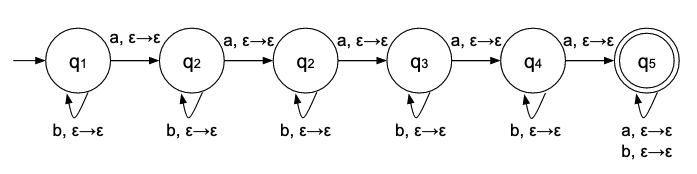
\includegraphics[width=0.95\textwidth]{4.png}
\end{center}

{\bf Question 5}\\

\begin{align*}
   & S \rightarrow ASA|AS|0A|\epsilon \\
   & A \rightarrow 001|\epsilon \\\\
   & \textbf{Add new start symbol}\\
   & S_0 \rightarrow S \\
   & S \rightarrow ASA|AS|0A|\epsilon \\
   & A \rightarrow 001|\epsilon \\\\
   & \textbf{Eliminate epsilon rules}\\
   & S_0 \rightarrow S \\
   & S \rightarrow ASA|AS|0A|\epsilon|S|SA|0 \\
   & A \rightarrow 001 \\\\
   & S_0 \rightarrow S|\epsilon \\
   & S \rightarrow ASA|AS|0A|S|SA|0|AA|A \\
   & A \rightarrow 001 \\\\
   & S_0 \rightarrow S|\epsilon \\
   & S \rightarrow ASA|AS|0A|SA|0|AA|A \\
   & A \rightarrow 001 \\\\
   & \textbf{Eliminate unit rules}\\
   & S_0 \rightarrow ASA|AS|0A|SA|0|AA|A|\epsilon \\
   & S \rightarrow ASA|AS|0A|SA|0|AA|A \\
   & A \rightarrow 001 \\\\
   & S_0 \rightarrow ASA|AS|0A|SA|0|AA|001|\epsilon \\
   & S \rightarrow ASA|AS|0A|SA|0|AA|001 \\
   & A \rightarrow 001 \\\\
   & \textbf{Convert remaining rules}\\
   & S_0 \rightarrow AW|AS|0A|SA|0|AA|001|\epsilon \\
   & S \rightarrow AW|AS|0A|SA|0|AA|001 \\
   & A \rightarrow 001 \\ 
   & W \rightarrow SA \\\\
\end{align*}

\begin{align*}
   & S_0 \rightarrow AW|AS|XA|SA|0|AA|001|\epsilon \\
   & S \rightarrow AW|AS|XA|SA|0|AA|001 \\
   & A \rightarrow 001 \\ 
   & W \rightarrow SA \\
   & X \rightarrow 0 \\\\
   & S_0 \rightarrow AW|AS|XA|SA|0|AA|XY|\epsilon \\
   & S \rightarrow AW|AS|XA|SA|0|AA|XY \\
   & A \rightarrow XY \\ 
   & W \rightarrow SA \\
   & X \rightarrow 0 \\
   & Y \rightarrow 01 \\\\
   & S_0 \rightarrow AW|AS|XA|SA|0|AA|XY|\epsilon \\
   & S \rightarrow AW|AS|XA|SA|0|AA|XY \\
   & A \rightarrow XY \\ 
   & W \rightarrow SA \\
   & X \rightarrow 0 \\
   & Y \rightarrow XZ \\
   & Z \rightarrow 1 \\
\end{align*}
G is now in Chomsky Normal Form.


\end{document}
